\documentclass[10pt,a4paper]{article}
\usepackage[utf8]{inputenc}
\usepackage[german]{babel}
\usepackage[T1]{fontenc}
\usepackage{amsmath}
\usepackage{amsfonts}
\usepackage{amssymb}
\usepackage{minted}
\usepackage[left=1cm, right=1cm, top=1cm, bottom=2cm]{geometry}
\usepackage{url}
\usepackage{graphicx}


\setcounter{section}{1}
\author{Julian Deinert, Tronje Krabbe}
\title{Labreport 05}
\linespread{0.5}
\begin{document}
\maketitle
\tableofcontents
\thispagestyle{empty}
\newpage
\setcounter{page}{1}


\section*{1. Netzwerkeinstellungen }
\addcontentsline{toc}{section}{1. Netzwerkeinstellungen}
\setcounter{subsection}{1}

\subsection{Ermitteln der Netzwerkkonfiguration}
\begin{itemize}
\item Die ClientVM hat die IP-Adresse \texttt{192.168.254.44} und das Standardgateway \texttt{192.168.254.2} außerdem verwendet sie den DNS-Server \texttt{10.1.1.1}.

\item Die RouterVM besitzt für das Interface \textit{eth0} die IP-Adresse \texttt{172.16.137.222} und für das Interface \textit{eth1} die IP-Adresse \texttt{192.168.254.2}.

\item Die ServerVM hat die IP-Adresse \texttt{172.16.137.144}.
\end{itemize}

\setcounter{section}{2}
\section*{2. Absichern eines Einzelplatzrechners mit iptables (ClientVM)}
\addcontentsline{toc}{section}{2. Absichern eines Einzelplatzrechners mit iptables (ClientVM)}
\setcounter{subsection}{0}
\subsection{Löschen aller Firewallregeln}

Wir richten die default policy wieder ein und flushen alle Chains  in der \textit{filter-}, \textit{nat-} und \textit{mangle-table}.
\begin{minted}{php}
# iptables -P INPUT ACCEPT
# iptables -P FORWARD ACCEPT
# iptables -P OUTPUT ACCEPT

# iptables -t nat -F
# iptables -t mangle -F
# iptables -F
# iptables -X
\end{minted}
Danach installieren wir mit \texttt{apt-get} das Paket \texttt{openssh-server}.

\subsection{Entwerfen eines Konzepts}
Wir wollen Traffic durch Port \texttt{80} und \texttt{443} generell erlauben und Traffic durch Port \texttt{22} nur aus dem lokalen Netzwerk zulassen. Hierzu setzen wir die folgenden IP-Table Einträge:
Zunächst ändern wir die defaults targets der drei chains \texttt{INPUT}, \texttt{OUTPUT} und \texttt{FORWARD} zu \texttt{DROP} (\texttt{REJECT} geht nicht;
der Versuch, \texttt{REJECT} als target zu nutzen endet mit der Fehlermeldung \textit{iptables: bad policy name. Run `dmesg' for more information.}).

\begin{verbatim}
# iptables -P INPUT DROP
# iptables -P OUTPUT DROP
# iptables -P FORWARD DROP
\end{verbatim}

Nun ist also gar keine Kommunikation mehr möglich. \texttt{ping} z.B. schlägt fehl mit \textit{ping: sendmsg: Operation not permitted}.
So weit, so gut. Nun wollen wir aber einige Kommunikation erlauben. Zunächst kümmern wir uns um \textit{ssh}:

\begin{verbatim}
# iptables -A INPUT -i eth0 -p tcp -s 192.168.254.0/24 --dport 22 -j ACCEPT
# iptables -A OUTPUT -o eth0 -p tcp --sport 22 -j ACCEPT
\end{verbatim}

Nach diesen Befehlen kann man sich aus dem lokalen 192.168.254er Netz auf die Client-VM per \textit{ssh} verbinden. Lässt man den \texttt{-s} Switch weg,
kann man sich von überall auf die VM \textit{ssh}en.

Nun brauchen wir noch HTTP (und HTTPS); wir erlauben eingehenden tcp traffic, der von einem Port 80 kommt,
und ausgehenden tcp traffic, der zu einem Port 80 will (bzw. Port 443 für HTTPS):

\begin{verbatim}
# iptables -A OUTPUT -o eth0 -p tcp --dport 80 -j ACCEPT
# iptables -A INPUT -i eth0 -p tcp --sport 80 -j ACCEPT

# iptables -A OUTPUT -o eth0 -p tcp --dport 443 -j ACCEPT
# iptables -A INPUT -i eth0 -p tcp --sport 443 -j ACCEPT
\end{verbatim}

Jetzt brauchen wir noch Regeln für ICMP:

\begin{verbatim}
# iptables -A INPUT -p icmp -j ACCEPT
# iptables -A OUTPUT -p icmp -j ACCEPT
\end{verbatim}

Wenn man lediglich z.B. pings (und pongs) erlauben will, würde man noch die \texttt{--icmp-type} flag auf einen entsprechenden
Wert setzen. In der Aufgabe wurde allerdings nur ``ICMP Nachrichten'' spezifiziert, also erlauben wir alles, was ICMP ist.

\subsection{Prüfen der Korrektheit der Regeln}
\begin{itemize}
\item Von der RouterVM aus können wir eine SSH-Verbindung zur ClientVM aufbauen. Von Client- zu RouterVM geht dies nicht.
	  Es soll ja nur eingehendes SSH erlaubt sein.
\item Wir starten einen netcat server in der ClientVM auf Port 5555 mit \texttt{nc -l 5555} (mit GNU netcat hätten wir noch die -p Flag nehmen müssen).
	  Jetzt versuchen wir, uns damit von der RouterVM aus zu verbinden: \texttt{nc 192.168.254.44 5555}. Komischerweise ergibt dies keine Fehlermeldung,
	  aber der netcat `client' terminiert nach einer kurzen Zeit. In dieser Zeit können keine Nachrichten ausgetauscht werden.
	  Dies ist natürlich gewollt; wir wollen nur HTTP(S), SSH und ICMP zulassen. Port 5555 hat mit keiner dieser Protokolle zu tun, und wird deshalb
	  nicht durchgelassen.
\item Da REJECT nicht als target für die default chains erlaubt ist, können wir dies nicht beobachten. REJECT verhält sich aber so:
	  Während DROP das Paket einfach fallen lässt (Zitat man-page: ``DROP means to drop the packet on the floor.''), sendet REJECT
	  noch eine Nachricht, dass das Paket eben rejected wurde.
\end{itemize}

\subsection{Stateful Filtering}
Zunächst: \texttt{\# iptables -F}.
Nun erlauben wir wieder SSH:

\begin{verbatim}
# iptables -A OUTPUT -o eth0 -p tcp -d 192.168.254.0/24 --dport 22 -m state --state NEW,ESTABLISHED -j ACCEPT
# iptables -A INPUT -i eth0 -p tcp --sport 22 -m state --state ESTABLISHED -j ACCEPT
\end{verbatim}
Nun beachten wir auch den state der Verbindung, und akzeptieren eingehende Pakete nur, wenn sie Teil einer bereits bestehenden Verbindung sind.
Ähnlich für HTTP(S):

\begin{verbatim}
# iptables -A OUTPUT -o eth0 -p tcp --dport 80 -m state --state NEW,ESTABLISHED -j ACCEPT
# iptables -A INPUT -i eth0 -p tcp --sport 80 -m state --state ESTABLISHED -j ACCEPT

# iptables -A OUTPUT -o eth0 -p tcp --dport 443 -m state --state NEW,ESTABLISHED -j ACCEPT
# iptables -A INPUT -i eth0 -p tcp --sport 443 -m state --state ESTABLISHED -j ACCEPT
\end{verbatim}

Die Regeln für ICMP bleiben gleich; hier gibt es keine bestehenden Verbindungen o.ä.
\\
\\
Stateful filtering kann flexibler und übersichtlicher sein. Man beachte folgende Regel:
\texttt{iptables -A INPUT -m conntrack --ctstate RELATED,ESTABLISHED -j ACCEPT}. Zusammen mit einer `DROP' policy
sichert sie ein System relativ gut ab. Eingehende Pakete werden nur akzeptiert, wenn sie bereits Teil einer etablierten oder verwandten
Verbindung sind.\\
Will man jedoch spezifischer filtern, kommt es immer darauf an, was genau erreicht werden soll; dann ist der state eines Pakets
nur eine weitere Variable, nach der gefiltert werden kann, und sollte nicht pauschal bevorzugt werden, wenn es nicht nötig ist.


\setcounter{section}{3}
\section*{3. Absichern eines Netzwerks (RouterVM)}
\addcontentsline{toc}{section}{3. Absichern eines Netzwerks (RouterVM)}
\setcounter{subsection}{0}

\subsection{Dynamisches NAT} % 3.1

Der \texttt{iptables} Aufruf in \textit{/etc/rc.local} lautet:
\begin{verbatim}
iptables -t nat -A POSTROUTING -o eth0 -s 192.168.254.0/24 -j MASQUERADE
\end{verbatim}
Der \texttt{-t nat} Switch wählt die \textit{nat} Table aus, der \texttt{-A POSTROUTING} Switch erstellt
eine neue Regel, um ausgehende Packets zu verändern. \texttt{-o eth0} wählt das Out-Interface aus, der 
\texttt{-s} Switch die Quell-Adresse. \texttt{-j MASQUERADE} spezifiziert das \texttt{MASQUERADE} target,
welches dafür sorgt, dass Traffic unverändert an das Interface fließt. Insgesamt sorgt die Regel also
dafür, dass Traffic aus dem \texttt{192.168.254.0/24} Netz zum \texttt{eth0} Interface durchgelassen wird.

\subsection{NAT-Abläufe} % 3.2
\begin{itemize}
    \item Wir können die ServerVM von der ClientVM aus \textit{ping}en.
    \item Von der ServerVM aus können wir nicht die ClientVM ansprechen, da die ServerVM im \texttt{172.16.137.0/24} Netz liegt.
        Tatsächlich kommen pings von der ServerVM in das \texttt{192.168.254.0/24} Netz scheinbar gar nicht in der RouterVM an.
        WireShark zeigt nämlich keine entsprechenden Pakete an. Von der ClientVM zur ServerVM werden die Request und Response
        Pakete korrekt aufgelistet (von Client zu Router, Router zu Server, und wieder zurück).
\end{itemize}

\subsection{IP-Tables} % 3.3

Wir filtern HTTP-Requests auf Port 80 und 443 nach \texttt{10.1.1.2} und \texttt{172.16.137.144} raus, und lassen alle anderen durch:
\begin{verbatim}
# iptables -A FORWARD -p tcp -d 10.1.1.2 --dport 80 -j DROP
# iptables -A FORWARD -p tcp -d 10.1.1.2 --dport 443 -j DROP
# iptables -A FORWARD -p tcp -d 172.16.137.144 --dport 80 -j DROP
# iptables -A FORWARD -p tcp -d 172.16.137.144 --dport 443 -j DROP
# iptabels -A FORWARD -p tcp -d 10.0.0.0/8 -j DROP
# iptables -A FORWARD -p tcp --dport 80 -m state --state NEW,ESTABLISHED,RELATED -j ACCEPT
# iptables -A FORWARD -j DROP
\end{verbatim}

\subsection{Anpassung für SSH-Verbindung} % 3.4

Wir möchten eine Verbindung zur ServerVM unter \texttt{172.16.137.144} auf Port \texttt{22} ermöglichen. Hierzu fügen wir an Stelle 7 eine neue Regel in die \textit{FORWARD CHAIN} ein. Wir lassen hier außerdem das Protokoll weg, damit auch UDP-Verbindungen möglich sind.
\begin{verbatim}
# iptables -I FORWARD 7 -d 172.16.137.144 --dport 22 -j ACCEPT
\end{verbatim}

\subsection{Weiterleitung 5022 auf 22} % 3.5

Wir leiten den Port \texttt{5022} der RouterVM auf den Port \texttt{22} der ClientVM weiter.
\begin{verbatim}
# iptables -t nat -A -p tcp --dport 5022 -j DNAT --to-destination 192.168.254.44:22 
\end{verbatim}

\subsection{Statische NAT-Regel} % 3.6

Wir wählen uns eine neue IP-Adresse aus dem gleichen Subnetz in der auch die ServerVM ist aus.
\begin{verbatim}
# ifconfig eth0:1 172.16.137.225 netmask 255.255.255.0
\end{verbatim}
Alle Anfragen auf die IP \texttt{172.16.137.225} sollen nun zur ClientVM durchgereicht werden.
\begin{verbatim}
# iptables -t nat -A PREROUTING -d 172.16.137.225 -j DNAT --to-destination 192.168.254.44
\end{verbatim}

\setcounter{section}{4}
\section*{4. SSH-Tunnel}
\addcontentsline{toc}{section}{4. SSH-Tunnel}
\setcounter{subsection}{0}

\subsection{Konfigurieren der Firewall}
\begin{verbatim}
# iptables -A FORWARD 0s 192.168.254.44 -d 172.16.137.144 -p tcp --dport 22 -j ACCEPT
# iptables -A FORWARD -s 192.168.254.44/32 -p udp -m udp --dport 53 -j ACCEPT
# iptables -A FORWARD -s 192.168.254.44/32 -j DROP
\end{verbatim}

\subsection{SSH-Tunnel}
Wir richten den SSH-Tunnel wie folgt ein.
\begin{verbatim}
$ ssh -L 8000:localhost:80 user@172.16.137.144
\end{verbatim}
Wireshark bestätigt die Korrektheit des Befehls.

\subsection{Tunnel ins Internet}
\begin{verbatim}
$ ssh -D licalhost:5555 user@172.16.137.144
\end{verbatim}
Konfiguration von Firefox im Appendix.

\subsection{Netcat}
Auf der ClientVM
\begin{verbatim}
$ nc -l 5555
$ ssh -R 8000:localhost:5555 user@172.16.137.144
\end{verbatim}
Um netcat auf Port \texttt{5555} lauschen zu lassen und einen Tunnel von ServerVM Port \texttt{8000} auf ClientVM Port \texttt{5555} einzurichten.

Dann, auf der ServerVM:
\begin{verbatim}
# nc localhost 8000
\end{verbatim}
Nun können wir beliebig Daten versenden.

\setcounter{section}{5}
\section*{5. OpenVPN}
\addcontentsline{toc}{section}{5. OpenVPN}
\setcounter{subsection}{0}
\subsection{Filter-Regeln}
\begin{verbatim}
# iptables -A FORWARD -s 192.168.254.0/24 -d 172.16.137.0/24 -j ACCEPT
# iptables -A FORWARD -j DROP
\end{verbatim}

\subsection{OpenVPN-Server einrichten}

Auf der ServerVM
\begin{verbatim}
$ openvpn --genkey --secret static.key
\end{verbatim}

\subsection{Filterregeln auf der ServerVM}
\begin{verbatim}
# iptables -A INPUT -p udp --dport 1194 -j ACCEPT
# iptables -A INPUT -j DROP
# iptables -A OUTPUT -p udp --dport 1194 -m conntrack --ctstate ESTABLISHED,RELATED -j ACCEPT
# iptables -A OUTPUT -j DROP
\end{verbatim}

\subsection{VPNClient}
Clientconfig im Appendix

\subsection{Starten des VPN-Tunnels}
Auf der ServerVM
\begin{verbatim}
$ sudo openvpn server.conf
\end{verbatim}
Auf der ClientVM
\begin{verbatim}
$ sudo openvpn client.conf
\end{verbatim}

\subsection{Funktionskontrolle}
Es wird das Interface \texttt{tun0} verwendet.
\begin{verbatim}
Wed Jun 22 19:50:12 2016 Peer Connection Initiated with [AF_INET]172.16.137.222:1194
Wed Jun 22 19:50:12 2016 Initialization Sequence Completed
\end{verbatim}
Über 10.8.0.1 können wir auf den Server zugreifen.
Wir könne von der ServerVM auf die ClientVM zugreifen, da der Tunnel bidirektional ist. Dies erreichen wir über die VPN-IP der ClientVM(10.8.0.2).
\setcounter{section}{6}
\section*{6. HTTP-Tunnel}
\addcontentsline{toc}{section}{6. HTTP-Tunnel}
\setcounter{subsection}{0}
\subsection{Neue Filterregeln}
Wir erlauben nur tcp Port \texttt{80} und udp Port \texttt{53}
\begin{verbatim}
# iptables -A FORWARD -s 192.168.254.44 -p tcp --dport 80 -j ACCEPT
# iptables -A FORWARD -s 192.168.254.44 -p udp --dport 53 -j ACCEPT
# iptables -A FORWARD -s 192.168.254.44 -j DROP
\end{verbatim}

\subsection{Umgehen der Filterrregeln}
Wir ändern in \texttt{etc/ssh/sshd\_config} den Port von \texttt{22} auf \texttt{80} und starten den Service mit \texttt{service ssh restart} neu, nachdem wir den bereits auf Port \texttt{80} laufenden Apache HTTP-Server gestoppt haben.

\subsection{Squid}



\newpage
\section*{Appendix}
\subsection*{4.3 Konfiguration von Firefox}
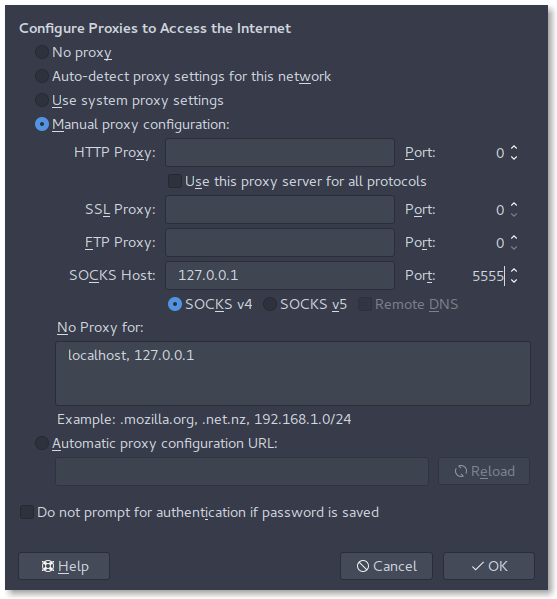
\includegraphics[width=\textwidth]{images/image.png}

\subsection*{5.2 OpenVPN Server Config}
\begin{verbatim}
port 1194
dev tun
ifconfig 10.8.0.1 10.8.0.2
secret static.key
keepalive 10 120
;status openvpn-status.log
verb 3
\end{verbatim}
\subsection*{5.2 OpenVPN Client Config}
\begin{verbatim}
dev tun
remote 172.16.137.144 1194
;resolve-retry infinite
;nobind
ifconfig 10.8.0.2 10.8.0.1
secret static.key
verb 3
\end{verbatim}
\end{document}
